\documentclass[tikz,border=5pt]{standalone}
\usepackage{amsmath, amssymb}
\usetikzlibrary{arrows.meta, calc}

\begin{document}
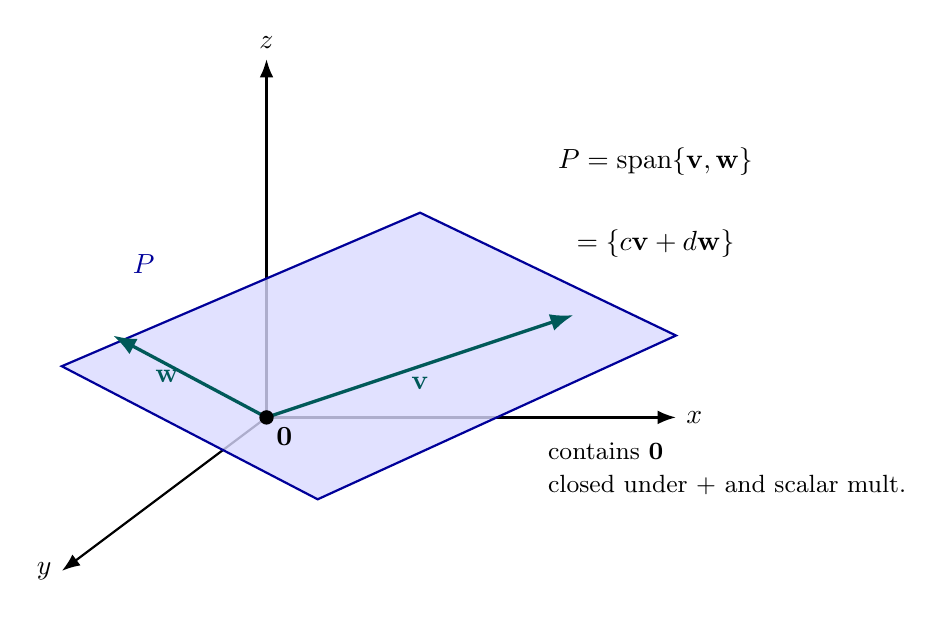
\begin{tikzpicture}[scale=1.3]

% Origen
\coordinate (O) at (0,0);

% Ejes (pseudo 3D)
\draw[-{Latex}, thick] (O) -- (4,0) node[right] {$x$};
\draw[-{Latex}, thick] (O) -- (-2,-1.5) node[left] {$y$};
\draw[-{Latex}, thick] (O) -- (0,3.5) node[above] {$z$};

% Plano generado por v y w
\fill[blue!15, opacity=0.8]
(-2,0.5) -- (1.5,2) -- (4,0.8) -- (0.5,-0.8) -- cycle;

\draw[blue!60!black, thick]
(-2,0.5) -- (1.5,2) -- (4,0.8) -- (0.5,-0.8) -- cycle;

% Vectores generadores
\draw[-{Latex}, very thick, teal!70!black] (O) -- (3,1)
node[midway, below] {$\mathbf{v}$};

\draw[-{Latex}, very thick, teal!70!black] (O) -- (-1.5,0.8)
node[midway, left] {$\mathbf{w}$};

% Origen
\fill (O) circle (2pt);
\node[below right] at (O) {$\mathbf{0}$};

% Texto clave (matemático)
\node at (3.8,2.5)
{$P = \text{span}\{\mathbf{v}, \mathbf{w}\}$};

\node at (3.8,1.7)
{$= \{c\mathbf{v} + d\mathbf{w}\}$};

% Etiqueta plano
\node[blue!60!black] at (-1.2,1.5) {$P$};

% Nota conceptual
\node[align=left] at (4.5,-0.5)
{\small contains $\mathbf{0}$ \\ \small closed under $+$ and scalar mult.};

\end{tikzpicture}
\end{document}